%FIXME mettre en évidence les définitions et propriétés ?
%FIXME pour les mathématiciens, donner de quoi le faire à la main : à partir de
%la séparation, montrer le paquet et donner le résumé qu'ils utiliseront

\title{Les tableaux}
\author{Guillaume \textsc{Huysmans}}%, Quentin \textsc{Carpentier}}
\date{2 décembre 2019}
\begin{document}
\maketitle

\begin{teacheronly}
\section*{Programme}
\subsection*{Compétences de 3TT en FWB}
\begin{tabular}{l|l}
10.1 & Analyser une situation-problème et
	modéliser la solution sous forme d'algorithme \\
10.5 & Traduire une opération, une fonction en langage de programmation \\
10.6 & Écrire un programme utilisant des séquences alternatives, répétitives \\
10.7 & Construire un programme modulaire \\
10.8 & Manipuler les tableaux
\end{tabular}
\subsection*{Prérequis}
J'ai déjà abordé la récursivité avec mes élèves lors d'une séance sur les tours
de Hanoï. Je les fais habituellement jongler entre deux notations : le
pseudo-code et le langage choisi en classe (ici, j'ai pris Python mais je ne
suis pas encore fixé).
\end{teacheronly}

\section{Introduction}

\emph{Le problème décrit ici dérive d'Advent of Code
\footnote{\url{https://adventofcode.com/2017/day/16}},
un calendrier de l'Avent avec
des problèmes algorithmiques au lieu de chocolats. Si vous en avez le courage,
essayez d'y participer cette année !}

Une société de petits personnages adore la danse. Chaque année, pour Noël, ils
organisent une grande fête à laquelle leur Grande Reine Vénérée participe. Sa
Majesté n'autorise pas tout et n'importe quoi : \tbold{seules les danses qui La
font commencer et finir à la première place sont permises.}
Si elle finit à une autre place, le
chorégraphe est exécuté. C'est ce qui est arrivé au chorégraphe de la Cour
l'année passée : il faut dire qu'avec son grand âge, il n'avait déjà plus toute
sa tête. Cette année, c'est à son fils de prendre la relève : tous les autres
ont bien trop peur de mourir pour un pas de travers. Il doit faire quelque
chose de grandiose s'il veut faire oublier l'erreur de son père et profiter de
ses cadeaux sous le sapin.
Le problème, c'est qu'il a laissé tomber ses papiers quelques
jours avant Noël et qu'il avait oublié de les numéroter.
Il a presque réussi à les remettre dans l'ordre mais \tbold{il hésite entre
deux possibilités} et il n'a plus le temps de \tbold{les essayer}.

Ils commencent dans l'ordre (${A\dots P}$) et enchaînent deux types de pas :
\begin{itemize}
\item \tbold{\texttt{spin}} $n$ ($\forall n \in \{1\dots15\}$) :
	\marginpar{expliquer la notation : $\forall x \in E$...}
	les \tbold{$n$ derniers} viennent devant les premiers. \\
	Par exemple, \texttt{spin 3} sur \texttt{DACB} donne \texttt{ACBD}.
\item \tbold{\texttt{exchange}} $i$ $j$ ($\forall i,j \in \{0\dots15\}$) :
	ceux en $i$ et $j$ échangent leur place. \\
	Par exemple, \texttt{exchange 0 2} sur \texttt{CBDA} donne \texttt{DBCA}.
\end{itemize}

\begin{exo}
\emph{Surlignez} les mots importants de l'histoire ci-dessus.
\end{exo}

Avec ce que nous avons déjà vu, il serait possible d'utiliser une variable par
case, donc deux fonctions avec plusieurs conditions suffiraient pour y lire et
y écrire mais ça devient vite pénible\footnote{Déjà avec 16 personnages...}.

Soient les variables $v_0, v_1, v_2\dots v_{15} \in\{A\dots P\}$.

\begin{exo}
\emph{Complétez} l'algorithme naïf \texttt{lire}$(i\in\{0\dots15\})$ :
\begin{enumerate}
\item si \pbox{$i=0$} alors retourner \pbox{$v_0$}
\item sinon, si \pbox{$i=1$} alors retourner \pbox{$v_1$}
\item sinon, si \pbox{$i=2$} alors retourner \pbox{$v_2$}
\item etc.
\end{enumerate}
\end{exo}

\begin{exo}
\emph{Complétez} l'algorithme naïf \texttt{écrire}$(i\in\{0\dots15\}, x)$ :
\begin{enumerate}
\item si \pbox{$i=0$} alors
	\pbox{$v_0$} $\leftarrow$ \pbox{$x\phantom{_0}$}
\item sinon, si \pbox{$i=1$} alors
	\pbox{$v_1$} $\leftarrow$ \pbox{$x\phantom{_0}$}
\item sinon, si \pbox{$i=2$} alors
	\pbox{$v_2$} $\leftarrow$ \pbox{$x\phantom{_0}$}
\item etc.
\end{enumerate}
\end{exo}

Remarquez que les \emph{indices} commencent à zéro !
\begin{exo}
\emph{Déterminez} l'indice du dernier élément d'un tableau de
$n\in\mathbb{N}_0$ éléments.
\end{exo}

Tout ce dont nous avons besoin, c'est d'accéder à la $i$ème variable.
Un tableau de $n\in\mathbb{N}$ éléments de type $\alpha$ est une
\emph{structure de données} qui permet précisément de le faire.
Cette structure propose deux opérations :
\begin{itemize}
\item \texttt{get}$(i\in\pbox{$\{0\dots n-1\}$}) : \alpha$ renvoie le $i$ème
	\marginpar{sens particulier de $\{0\dots n-1\}$}
	élément du tableau. \\
	En Python : \texttt{t[i]}
\item \texttt{set}$(i\in\pbox{$\{0\dots n-1\}$}, x\in\alpha)$ remplace le
	$i$ème élément par $x$ et ne renvoie rien. \\
	En Python : \texttt{t[i] = x}
\end{itemize}

Nous adopterons une notation graphique pour les représenter, même si \emph{un
programme ne verra pas (contrairement à nous) directement où se trouve chaque
élément} :
\marginpar{couleurs dans leur dos pour ne pas les voir direct'}
\newcommand{\boxes}[4]{
	$\begin{array}{|l|l|l|l|}\hline
	\ptonly{#1} & \ptonly{#2} & \ptonly{#3} & \ptonly{#4} \\ \hline
	\end{array}$
}
\newcommand{\emptyboxes}{
	\boxes{\phantom{a}}{\phantom{a}}{\phantom{a}}{\phantom{a}}
}
\begin{equation*}
	\texttt{['a', 'b', 'c', 'd']} \equiv
	\begin{array}{|l|l|l|l|}\hline
		a & b & c & d \\ \hline
	\end{array}
\end{equation*}

En Python\footnote{Ce n'est pas vrai dans tous les langages de programmation.},
un tableau peut changer de taille au cours de l'exécution du programme :
\begin{itemize}
\item \texttt{[]} est un \emph{nouveau} tableau vide.
	\marginpar{sinon plus possible d'utiliser \texttt{[]}
	après \texttt{[].append}}
\item \texttt{t.append(x)} ajoute un élément à la fin de \texttt{t}.
\item \texttt{len(t)} retourne la longueur de $t$.
\end{itemize}
Cependant, faites attention aux indices ! Si vous accédez à un indice qui
n'existe pas, votre programme pourrait se planter. Ou pire.

\begin{exo}[Bonus]
\emph{Demandez} à Python si \texttt{[] is []} est vrai,
puis \emph{essayez} avec des nombres...
\end{exo}

\begin{exo}
\emph{Tapez} les instructions suivantes dans le
REPL\footnote{\emph{Read-Eval-Print Loop}} et
\emph{expliquez} chaque résultat :
\begin{enumerate}
	\item \texttt{t = []} \tonly{crée un tableau vide}
		\hfill \boxes ////
	\item \texttt{print(t[0])} \tonly{lève une \texttt{IndexError}}
	\item \texttt{t.append(2)}
		\hfill \boxes 2///
	\item \texttt{print(t[0])} \tonly{affiche 2, le premier élément}
	\item \texttt{print(t[-1])} \tonly{devrait les surprendre}
	\item \texttt{t.append(4)}
		\hfill \boxes 24//
	\item \texttt{print(t[-1])} \tonly{affiche 4, le dernier élément}
	\item \texttt{t.append(6)}
		\hfill \boxes 246/
	\item \texttt{t.append(8)}
		\hfill \boxes 2468
	\item \texttt{print(t[-2])} \tonly{affiche 6, l'avant-dernier élément}
	\item \texttt{print(t[1.5])} \tonly{lève une \texttt{TypeError}}
\end{enumerate}
\end{exo}

\section{Simulation}
Pour simplifier, limitons-nous à 4 personnages
représentés par quatre lettres.

\begin{exo}\label{ex:sim}
\emph{Simulez} les étapes successives de cette danse :
	\begin{enumerate}%[label=\alph*.]
	\item (positions initiales) \hfill \boxes abcd
	\item \texttt{spin 3} \hfill \boxes bcda
	\item \texttt{exchange 0 1} \hfill \boxes cbda
	\item \texttt{spin 1} \hfill \boxes acbd
	\item \texttt{exchange 2 3} \hfill \boxes acdb
	\end{enumerate}
\end{exo}

\begin{exo}
\emph{Complétez} ces schémas puis \emph{implémentez} \texttt{exchange} :
	\marginpar{cases vides !!}
\begin{multicols}{2}
	\begin{enumerate}[label=]
	\item \emptyboxes \texttt{spin$(n\in\{1\dots4\})$}
	\item \emptyboxes \texttt{exchange$(i, j\in\{0\dots3\})$}
	\end{enumerate}
\end{multicols}
\end{exo}

\begin{exo}
En permutant deux pas, le résultat change...
	(\emph{entourez et justifiez} la bonne réponse) :
	\begin{enumerate}
		\item toujours ?
			\tonly{$x_{01}\circ x_{23}=x_{23}\circ x_{01}\equiv$\boxes badc}
			\marginpar{détailler une fois au tableau}
		\item jamais ?
			\tonly{$x_{01}\circ x_{12}\equiv$\boxes cabd$\ne$
			\boxes bcad$\equiv x_{12}\circ x_{01}$}
		\item parfois ? \tonly{parce qu'on a contredit les deux précédentes !}
	\end{enumerate}
\end{exo}

\begin{exo}
Schématisez une manière d'aider notre chorégraphe favori.
\begin{enumerate}
\item \tonly{Exécuter la première possibilité.}
\item \tonly{Tester \texttt{t[-1] == 'a'}.}
\item \tonly{Si c'est vrai, c'est la bonne, sinon, c'est l'autre.}
\end{enumerate}
\end{exo}

Remarquez qu'aucun personnage ne peut disparaître du tableau.
\begin{exo}
\emph{Écrivez} l'algorithme
\texttt{trouve}$(i\in\{0\dots15\}, x\in\{A\dots P\})$ qui retrouve la position
d'un personnage dans notre simulation en commençant par la $i$ème case.
\begin{enumerate}
\item \tonly{Si \texttt{t[i] == x}, retourner $i$.}
\item \tonly{Sinon, poursuivre la recherche à partir de l'indice $i+1$.}
\end{enumerate}
\end{exo}
\begin{exo}[Préparation]
	\emph{Expliquez} comment corriger une danse. \marginpar{\texttt{exchange}}
\end{exo}

\section{Optimisations}
\begin{comment}
Grâce à vous, Noël se passera bien pour notre ami.
Il nous doit une \emph{reconnaissance éternelle}
mais il a encore un <<~petit quelque chose~>> à nous demander.

Il a entendu dire que
Sa~Majesté se lassait de tout ça et qu'elle avait décidé de changer les règles :
pendant le prochain milliard d'années (ils vivent tous très longtemps mais la
principale cause de mortalité est la décapitation), l'Élu
(qu'Elle essaiera de ne pas exécuter entre-temps, Elle fera un effort)
participera à sa place et ils reprendront du même endroit l'année suivante.
%Grâce à ses talents de négociateur, il a pu obtenir de Sa~Majesté qu'elle
%accepte plus de danses originales (Elle n'est plus toujours première à la fin)
%à condition qu'après un milliard d'années, Elle finisse à nouveau la première.
La danse ne changera pas (quel intérêt si Elle ne regarde pas ?).
Le chorégraphe doit maintenant prédire la position exacte des danseurs après
tout ce temps. S'il se trompe, il sera exécuté, lui et toute sa famille.
%Son règne n'est pas près de s'arrêter : Sa~Majesté est immortelle.
\end{comment}

\subsection{Périodicité}
Si on écrit $d(x)$ le résultat de la danse $d$ sur les positions des danseurs
$x$, les positions à la fin de chaque danse peuvent être modélisées à l'aide
d'une suite :\[
	\forall n \in \mathbb{N} \quad u_n =
	\left\{\begin{array}{ll}
		\texttt{ABCDEFGHIJKLMNOP} & \text{si $n=0$} \\
		d\left(u_{n-1}\right) & \text{sinon}
	\end{array}\right.
\]

\emph{Il se peut} qu'il ne soit pas nécessaire de calculer $u_{1000000000}$ :
\begin{center}
	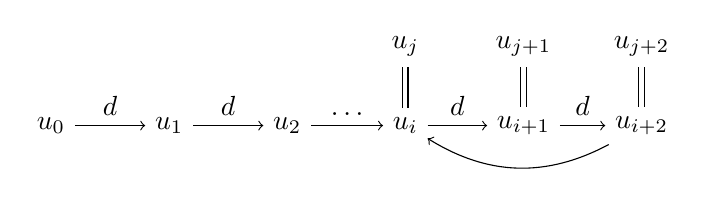
\begin{tikzpicture}[node distance=1.5cm]
		\node (0) {$u_0$};
		\node (1) [right of=0] {$u_1$};
		\node (2) [right of=1] {$u_2$};
		\node (i) [right of=2] {$u_i$};
		\node (i+1) [right of=i] {$u_{i+1}$};
		\node (i+2) [right of=i+1] {$u_{i+2}$};
		\node (j) [above of=i,node distance=1cm] {$u_j$};
		\node (j+1) [above of=i+1,node distance=1cm] {$u_{j+1}$};
		\node (j+2) [above of=i+2,node distance=1cm] {$u_{j+2}$};
		\draw (0) edge[->] node [above,midway] {$d$} (1);
		\draw (1) edge[->] node [above,midway] {$d$} (2);
		\draw (2) edge[->] node [above,midway] {$\dots$} (i);
		\draw (i) edge[->] node [above,midway] {$d$} (i+1);
		\draw (i+1) edge[->] node [above,midway] {$d$} (i+2);
		\draw (i+2) edge[->,bend left] node [below,midway] {} (i);
		%\draw (j) edge[->] node [above,midway] {$d$} (j+1);
		%\draw (j+1) edge[->] node [above,midway] {$d$} (j+2);
		%\draw (j+2) edge[->,bend right] node [above,midway] {$\dots$} (j);
		\draw (i) edge[double equal sign distance] (j);
		\draw (i+1) edge[double equal sign distance] (j+1);
		\draw (i+2) edge[double equal sign distance] (j+2);
	\end{tikzpicture}
\end{center}

\begin{exo}
À partir du dessin, \emph{déduisez} $k$, la période de la danse.
\begin{equation*}
k=\pbox{2+1=3}
\end{equation*}
\end{exo}

En pratique, la période pourrait être assez longue, c'est pourquoi \emph{on ne
stockera pas toutes les valeurs en mémoire}.
Ce problème a déjà été étudié %en théorie des graphes (un graphe est un ensemble
%de \emph{points} ou \emph{noeuds} reliés par \emph{arêtes})
par des mathématiciens
et nous allons redécouvrir l'\emph{algorithme du lièvre et de la tortue}.

Imaginons une course entre un lièvre et une tortue sur le parcours formé par
$u_n$. Évidemment, le lièvre court plus vite que la tortue (disons deux fois
plus vite). Dans cette course, avancer correspond à effectuer toute une danse
(de notre problème initial).

\begin{exo}
Avec votre voisin, faites la course sur le dessin (pour l'exemple, disons que
$i=3$) et \emph{retrouvez} la période $k$ à partir de vos positions respectives.
\end{exo}

\begin{exo}[Préparation]
\emph{Essayez} d'implémenter la simulation de cette course.
\end{exo}

\subsection{Ça tourne...}

\begin{exo}[Préparation]
\emph{Représentez} les personnages sur un cercle.
\end{exo}

\begin{exo}
\emph{Répondez} aux questions suivantes :
\begin{enumerate}
\item Où se trouve le premier danseur ?
	\marginpar{flèche}
\item Y a-t-il plusieurs façons de lire un tel schéma ?
	\marginpar{sens de rotation}
\item Que fait \texttt{spin 2} ? Est-ce que ça va plus vite ?
	\marginpar{compter à partir de la flèche}
\item Que fait \texttt{exchange 0 3} après \texttt{spin 2} ?
\item Un tableau est-il encore adapté ?
	\marginpar{plier, montre.}
	\begin{itemize}
	\item Si c'est le cas, représentez-le à plat.
	\item Sinon, expliquez pourquoi c'est impossible.
	\end{itemize}
\end{enumerate}
\end{exo}

\begin{teacheronly}
\section*{La suite}
La véritable préparation notée au journal de classe dépendra de l'avancement de
la classe.

Pour réellement implémenter la simulation, plusieurs approches sont
envisageables :
\begin{itemize}
\item \emph{parser} les pas stockés dans un fichier texte semblable à ce qui
	est produit par le générateur original : le code n'est pas particulièrement
	compliqué mais autant évaluer une chose à la fois. Même en BAB1, c'est non
	trivial (cf. séance CPUMONS).
\item générer une longue fonction qui effectue une danse : ce n'est pas d'une
	grande élégance mais ça a le mérite d'être transparent et plus facile à
	déboguer. Un autre avantage de cette approche est qu'elle leur montre
	qu'une optimisation peut être non triviale.
\end{itemize}

La notion de \emph{type somme}
\footnote{En OCaml, \texttt{type t = Spin of int | Exchange of int * int}}
(avec le \emph{pattern matching}
\footnote{\texttt{match s with Spin n -> ... | Exchange (i, j) -> ...}}) peut
aider à mieux structurer le programme et montre une alternative à la POO au
moins aussi élégante.

Pour faire du dépassement, j'ai le choix entre différents parcours :
\begin{itemize}
\item un peu de programmation fonctionnelle pour exhiber
	la composition de fonctions
\item seconde partie avec une nouvelle opération
	\texttt{partner}$(x, y\in\{A\dots P\})$
\end{itemize}
\end{teacheronly}

\end{document}
